\documentclass{article}
\usepackage[utf8]{inputenc}
\usepackage{a4wide}
\usepackage[T1]{fontenc}
\usepackage[french]{babel}
\usepackage[babel=true]{csquotes} % guillemets français
\usepackage{graphicx}
\graphicspath{{Images/}}
\usepackage{color}
\usepackage{hyperref}
\hypersetup{colorlinks,linkcolor=,urlcolor=blue}

\usepackage{amsmath}
\usepackage{amssymb}

\title{Sécurité Informatique}
\author{HOARAU Julien }
\date{April 2020}

\begin{document}

\maketitle

\section{Introduction}
Le But du projet est de créer une application mobile sur la plateforme Android ou swift basé sur la Cryptographie. En effet, nous avons plusieurs algorithmes à coder comme : Atbash, César, Vigenère, Hill, le carré de Polybe, Playfair, la Transposition rectangulaire, le DES (Data Encryption Standard), et le RSA.
Dans ce projet, nous allons voir l'ensemble de ses algorithmes codé sur la plateforme iOS avec leurs difficultées et futur amélioration.
Certain de ses Algorithmes, sont appliqués sur la table \textit{ASCII étendu} .\newline
Tout au long de ce projet, nous utilisons la table ASCII étendu : ISO/IEC 8859-1
Nous allons voir dans un premier temps les différents Algorithmes avec leur principe de fonctionnement et les difficultés que j'ai rencontré.
Puis nous allons voir les difficultés rencontrées en général.


\section{Sommaire}
\begin{enumerate}
\item Atbash
\item César
\item Vigenère 
\item Carré de Polybe
\item Playfair
\item Hill
\item Transposition Rectangulaire
\item DES
\item RSA
\end{enumerate}
\newpage
\section{Atbash}
\subsection{Principe}
Atbash est un chiffrement par subtitution monoalphabétique simple pour l'alphabet hébreu. Cette méthode consiste a subtitué la premiere lettre de l'alphabet (a) avec la dernière (z) puis la deuxième lettre avec l'avant dernière (y) ect ...

\subsection{Dans le code}
Dans l'application, Atbah est appliquée sur la table ASCII étendu.\newline
En effet, l'algorithme se base s'appuie sur les 256 valeurs de la table.
\begin{verbatim}
func atbash(t : [Int]) -> [Int]{//modifie les valeur ascii (atbash)
        print("Valeur Ascii du message : ",t)
        var tab : [Int] = []
        for i in t {
            let x = 256 - 1 - i //func atbash : f(x) = taille du tableau - 1 - index
            tab.append(x)
        }
        return tab
    }
\end{verbatim}
Cette fonction, codée sous le langage, nous renvoie la valeur opposée dans la table ASCII étendu. On remarque que la fonction manipule des entiers, effectivement, il y a une fonction qui permet de stocker dans un tableau les valeurs entières des caractères saisie : 
\begin{verbatim}
    func getAsciiInt(m : String) -> [Int]{
        print("message clair : ",m)
        var tab : [Int] = []
        let mess = Array(m)
        var i = 0
        while i <= (mess.count - 1){
            if mess[i] == "\\" && i < mess.count - 1 {/
                if mess[i+1] == "x" {
                    print("Détection de l'Hexa")
                    var hex : String = ""
                    i += 2 //on saute le \x
                    var j = 0
                    while j != 2 {
                        print("lettre hexa : ",mess[i])
                        hex.append(mess[i])
                        i += 1
                        j += 1 //compteur pour l'hexadécimal
                    }
                    tab.append(Int(hex, radix: 16)!)
                }
            }else{
                tab.append(Int(UnicodeScalar(String(mess[i]))!.value))
                i += 1
            }
        }
        return tab
    }
\end{verbatim}
On peut remarquer que cette fonction stocke chaque caractère par sa valeur entière correspondante dans la table ASCII. De plus, on s'aperçoit qu'une partie de la fonction permet de détecter la présence de l'hexadécimal représenté par :

\begin{verbatim}
    \x
\end{verbatim} et deux caractères qui se suivent (00 à ff : 0 à 256 valeurs)


 Il existe aussi une autre fonction qui permet de faire le fonctionnement inverse de GetAsciiInt, c'est la fonction getAsciiChar. Elle permet de faire la liaison entre le Symbole et sa valeur Entière. On notifie aussi qu'elle détecte les valeurs hexadécimale.

\subsection{Difficultées:}

Les difficultés rencontrées étaient de pouvoir lire la valeur entière du caractère saisies, mais aussi de connaître le caractère entrée selon la valeur décimal.\newline De plus, le format des valeurs Hexadécimales ont été créer pour être conforme à celle de l'énoncé.
\newpage
\section{César}
\subsection{Principe}
Le chiffrement de César est une méthode de chiffrement très simple.
Le texte chiffré s'obtient en remplaçant chaque lettre du texte clair original par une lettre à distance fixe, toujours du même côté, dans l'ordre de l'alphabet. Pour les dernières lettres (dans le cas d'un décalage à droite), on reprend au début. Par exemple avec un décalage de 3 vers la droite, A est remplacé par D, B devient E, et ainsi jusqu'à W qui devient Z, puis X devient A etc.

\subsection{Dans le code}
\begin{verbatim}
    func CrypCesar(cle : Int, t: [Int]) -> [Int]{
        var tab : [Int] = []
        let modulo = 256
        for i in t {
            tab.append((i+cle)%modulo)
        }
        return tab
    }
    
    func DecrypCesar(cle : Int, t: [Int]) -> [Int]{
        var tab : [Int] = []
        let modulo = 256
        for i in t {
            tab.append((i-cle)%modulo)
        }
        return tab
    }
\end{verbatim}
Nous voyons au-dessus les deux fonctions principales afin de coder et de décoder un message.
Dans le ViewController vous pouvez apercevoir que l'algorithme est appliqué sur la table ASCII mais aussi que certaines fonctions sont identique à celle de Atbash.
\newline Effectivement les fonctions GetAsciiInt et getAsciiChar seront présent dans tous les algorithmes manipulant des caractères dans la table ASCII.

\subsection{Difficultés:}
Je n'ai pas rencontré de difficulté particulière pour cet algorithme.

\newpage

\section{Vigenère}
\subsection{Principe:}
Le chiffre de Vigenère est un système de chiffrement par substitution polyalphabétique mais une même lettre du message clair peut, suivant sa position dans celui-ci, être remplacée par des lettres différentes, contrairement à un système de chiffrement mono alphabétique comme le chiffre de César (qu'il utilise cependant comme composant).\newline
Ce chiffrement introduit la notion de clé. Une clé se présente généralement sous la forme d'un mot ou d'une phrase. Pour pouvoir chiffrer notre texte, à chaque caractère nous utilisons une lettre de la clé pour effectuer la substitution. Évidemment, plus la clé sera longue et variée et mieux le texte sera chiffré. Il faut savoir qu'il y a eu une période où des passages entiers d'œuvres littéraires étaient utilisés pour chiffrer les plus grands secrets.
\subsection{Dans le code : }
Pour chiffrer un message, l'algorithme de Vigenère s'appuie sur une clé comme mentionnée ci-dessus. Nous pouvons avoir plusieurs cas lors de la saisie du message et de la clé. \newline
Effectivement, nous pouvons avoir le cas : 
\begin{itemize}
\item La taille du message est identique a la taille de la clé. 
\end{itemize}
On a aucune modification à faire.
\begin{itemize}
\item La taille du message est supérieur a la taille de la clé. 
\end{itemize}
On répète la clé pour quelle a la même taille que le message.
\begin{verbatim}
    func repeatKey(m : String, k : String) -> String{
        var rk : String = k //clé qui va etre répété
        if m.count > k.count{
            let tm = Array(m)
            let tk = Array(k)
            var i = tk.count
            while i < tm.count {
                rk.append(tk[i % tk.count])
                i += 1
            }
            
        }
        return rk
    }
\end{verbatim}
\newpage
Les fonctions utilisées pour déchiffrer et chiffrer :
\begin{center}
  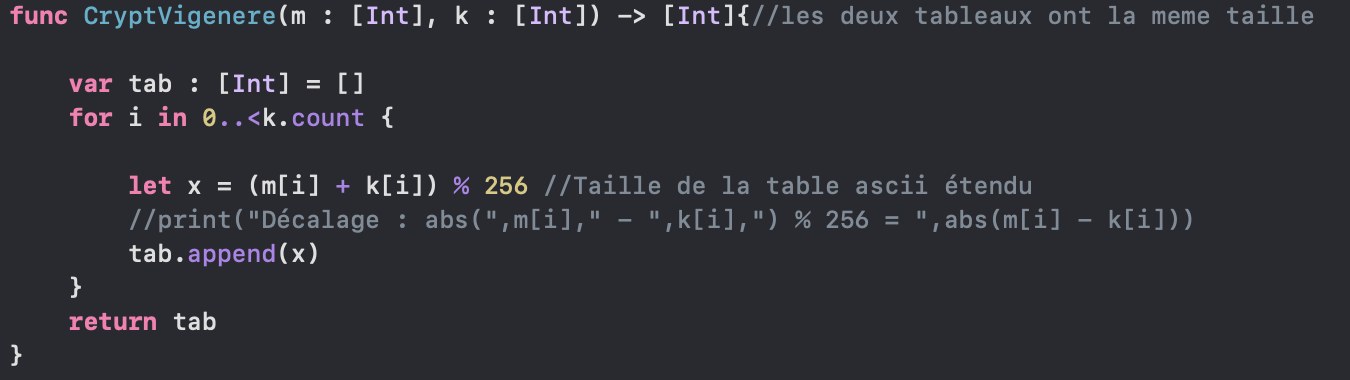
\includegraphics[scale=0.5]{Images/VigenereC.png}
  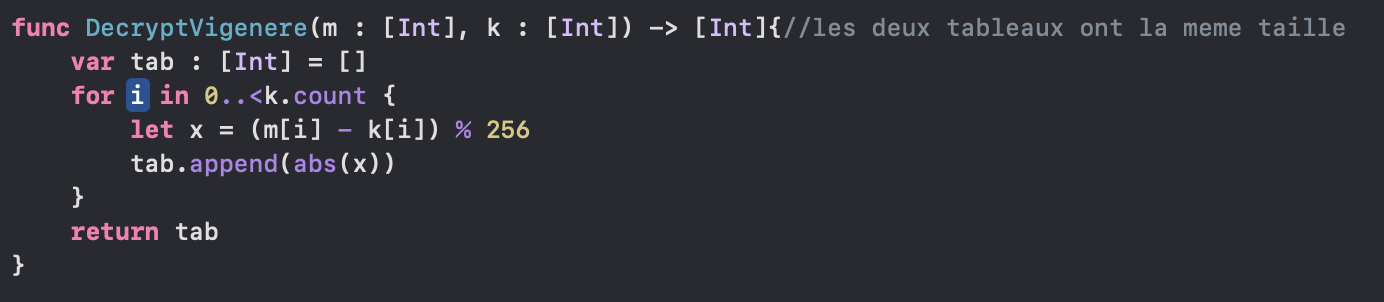
\includegraphics[scale=0.5]{Images/VigenereD.png}
\end{center}
\subsection{Difficultés:}
Je n'ai pas rencontré de difficulté particulière pour cet algorithme.
\newpage
\section{Carré de Polybe}
\subsection{Principe: }
Le principe est assez simple, il consiste à ordonner les lettres de l’alphabet en ordre alphabétique dans un tableau carré de 6 cases de côté dont chaque ligne et chaque colonne sont numérotées, de gauche à droite et de haut en bas. Considérant que l’alphabet français comporte 26 lettres et que le carré possède seulement 36 cases, on peut rajouter les 10 chiffres (0 à 9)

Ensuite, pour chiffrer un mot, il faut trouver la paire de numéros correspondants à chaque lettre. Le premier chiffre est le numéro de la colonne et le second celui de la rangée.

\subsection{Dans le code:}
Cet algorithme n'est pas appliqué sur l'ASCII, mais que sur 36 caractères : "abcdefghijklmnopqrstuvwxyz1234567890"\newline
\begin{verbatim}
     func CreateSquarePolybe() -> [Array<String>] {//Créer le tableau Polye de 36 charactère de a à 0
        let alpha = "abcdefghijklmnopqrstuvwxyz1234567890"
        //print(alpha.count)
        let tab = Array(alpha)
        var t : [Array<String>] = []
        var index = 0
        for _ in 0...5{
            var x : [String] = []
            for _ in 0...5{
                x.append(String(tab[index]))
                index += 1
            }
            t.append(x)
        }
        //print(t)
        return t
    }
\end{verbatim}
La fonction Createsquare permet de créer le carré de polybe.
Puis nous avons d'autres fonctions qui permettent de lire le tableau.
\begin{itemize}
    \item GetNumber prend en paramètre le tableau de polybe et un caractère, elle retourne la ligne puis la colonne.
    \item GetLetter prend en paramètre un x et qui va correspondre a la ligne puis a la colonne du tableau.
    
\end{itemize}
GetNumber prend en paramètre le tableau de polybe et un caractère, il retourne la ligne puis la colonne. La fonction va retourner le caractère correspondant dans le tableau.

\subsection{Difficultés:}
Je n'avais pas de difficulté particulière pour cet algorithme 

\section{Playfair}
\subsection{Principe :}
Le Chiffre de Playfair ou Carré de Playfair est une méthode manuelle de chiffrement symétrique qui fut la première technique utilisable en pratique de chiffrement par substitution polygrammique.\newline
Il consiste à chiffrer des paires de lettres (des digrammes), plutôt que des lettres seules comme dans les chiffrements par substitutions poly-alphabétiques tels que le chiffre de Vigenère.\newline
Le chiffre de Playfair utilise un tableau de 6*6 lettres, contenant un mot clé ou une phrase. La mémorisation du mot clé et de 4 règles à suivre suffisent pour utiliser ce chiffrement.
\subsection{Dans le code:}
On remarquera que certaines fonctions sont similaires comme dans le code du carré de polybe. En effet, nous avons les mêmes fonctions pour parcourir la table.\newline
En revanche, la création du tableau est similaire à celle de Polybe. La différence est qu'on complète le tableau avec la clé tout évitant les occurrences.
\begin{verbatim}
    func CreateTablePlayfair(k : String) -> [String]{
        let key = Array(k)
        let alpha = Array("abcdefghijklmnopqrstuvwxyz1234567890")
        var tab : [String] = []
        var i = 0
        while i < key.count {
            //élimine les occurences
            if !tab.contains(String(key[i])) && key[i] != " "{ 
                tab.append(String(key[i]))
            }
            i += 1
        }
        //print("tab with only key : \(tab)")
        var j = 0
        while j < alpha.count {
            //éliminé les espaces et les récurrences
            if !tab.contains(String(alpha[j])) && alpha[j] != " "{ 
                tab.append(String(alpha[j]))
            }
            j += 1
        }
        //print("tab : \(tab)")
        return tab
    }
\end{verbatim}
\subsection{Difficultés :}
Je n'avais pas de difficulté particulière pour cette algorithme

\section{Hill}
\subsection{Principe :}
Il consiste à chiffrer le message en substituant les lettres du message, non plus lettre à lettre, mais par groupe de lettres.l permet ainsi de rendre plus difficile le cassage du code par observation des fréquences.
Les lettres sont regroupées par lettre de 2,puis transcrit par leur valeur entière dans la table Ascii. La clé est une matrice 2,2 qui permettra de chiffre le message.
\subsection{Dans le code:}
La première fonction que nous allons voir est la fonction CanBeUseHill.
Cette fonction a pour but de vérifier si la matrice est conforme afin qu'elle puisse être utilisée pour chiffrer et déchiffrer par la suite. Concrètement on regarde si le pgcd de :
(a*d - b*c) est égale 1. Si oui la matrice est conforme, sinon on arrête l'algorithme.
\newline Ensuite nous allons nous pencher sur la fonction qui permet de déchiffrer :
 \begin{center}
     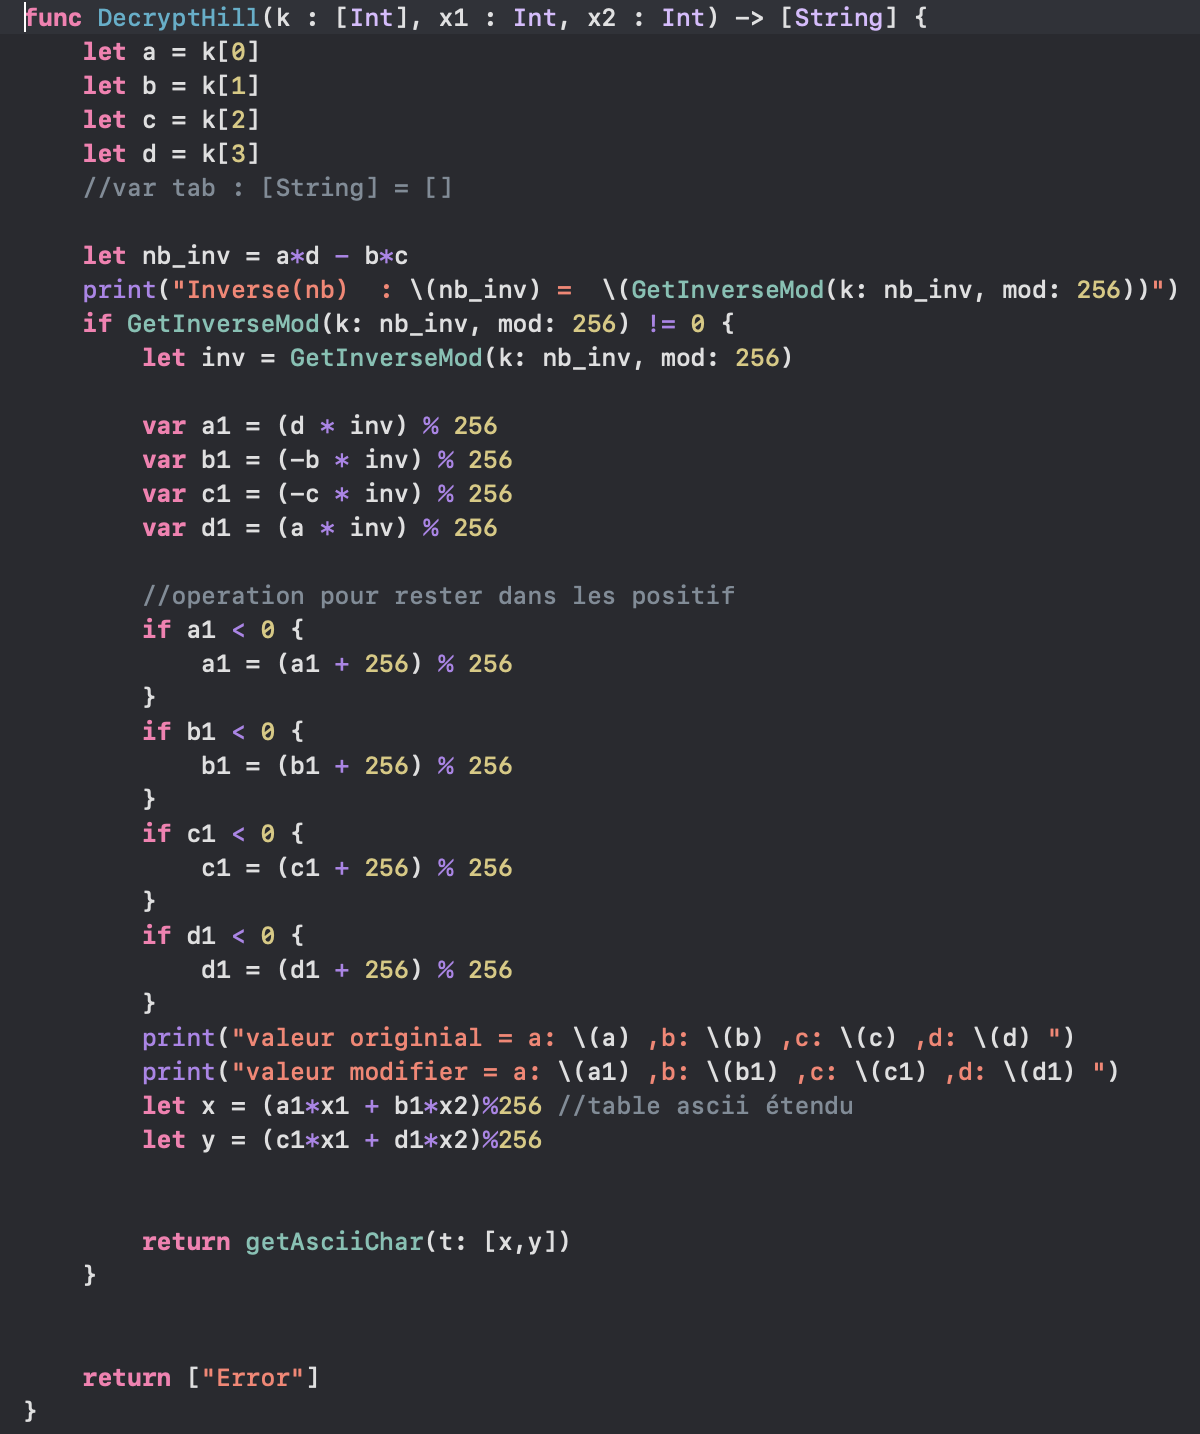
\includegraphics[scale=0.5]{HillD.png}
 \end{center}
 Dans cette fonction, on peut apercevoir l'utilisation d'une autre fonction GetInversMod.
 Elle permet d'avoir l'inverse du modulo afin de pouvoir décrypter le message chiffré sur 255.

\subsection{Difficultés :}
La plus grande difficulté était de comprendre le code et de pouvoir l'appliqué sur la table ASCII étendu.En effet, j'ai du j'ai cherché un algorithme qui permettait de calculer l'inverse modulaire puis l'adapter aux langage Swift.
\newpage
\section{Transposition Rectangulaire}
\subsection{Principe :}
Une transposition rectangulaire consiste à écrire le message dans une grille rectangulaire, puis à arranger les colonnes de cette grille selon un mot de passe donné (le rang des lettres dans l'alphabet donne l'agencement des colonnes)
\subsection{Dans le code:}
Dans ce code, le tableau est inspiré du code du playfair. En effet on insére la clé plus le message mais tout en laissant les occurences.
\begin{center}
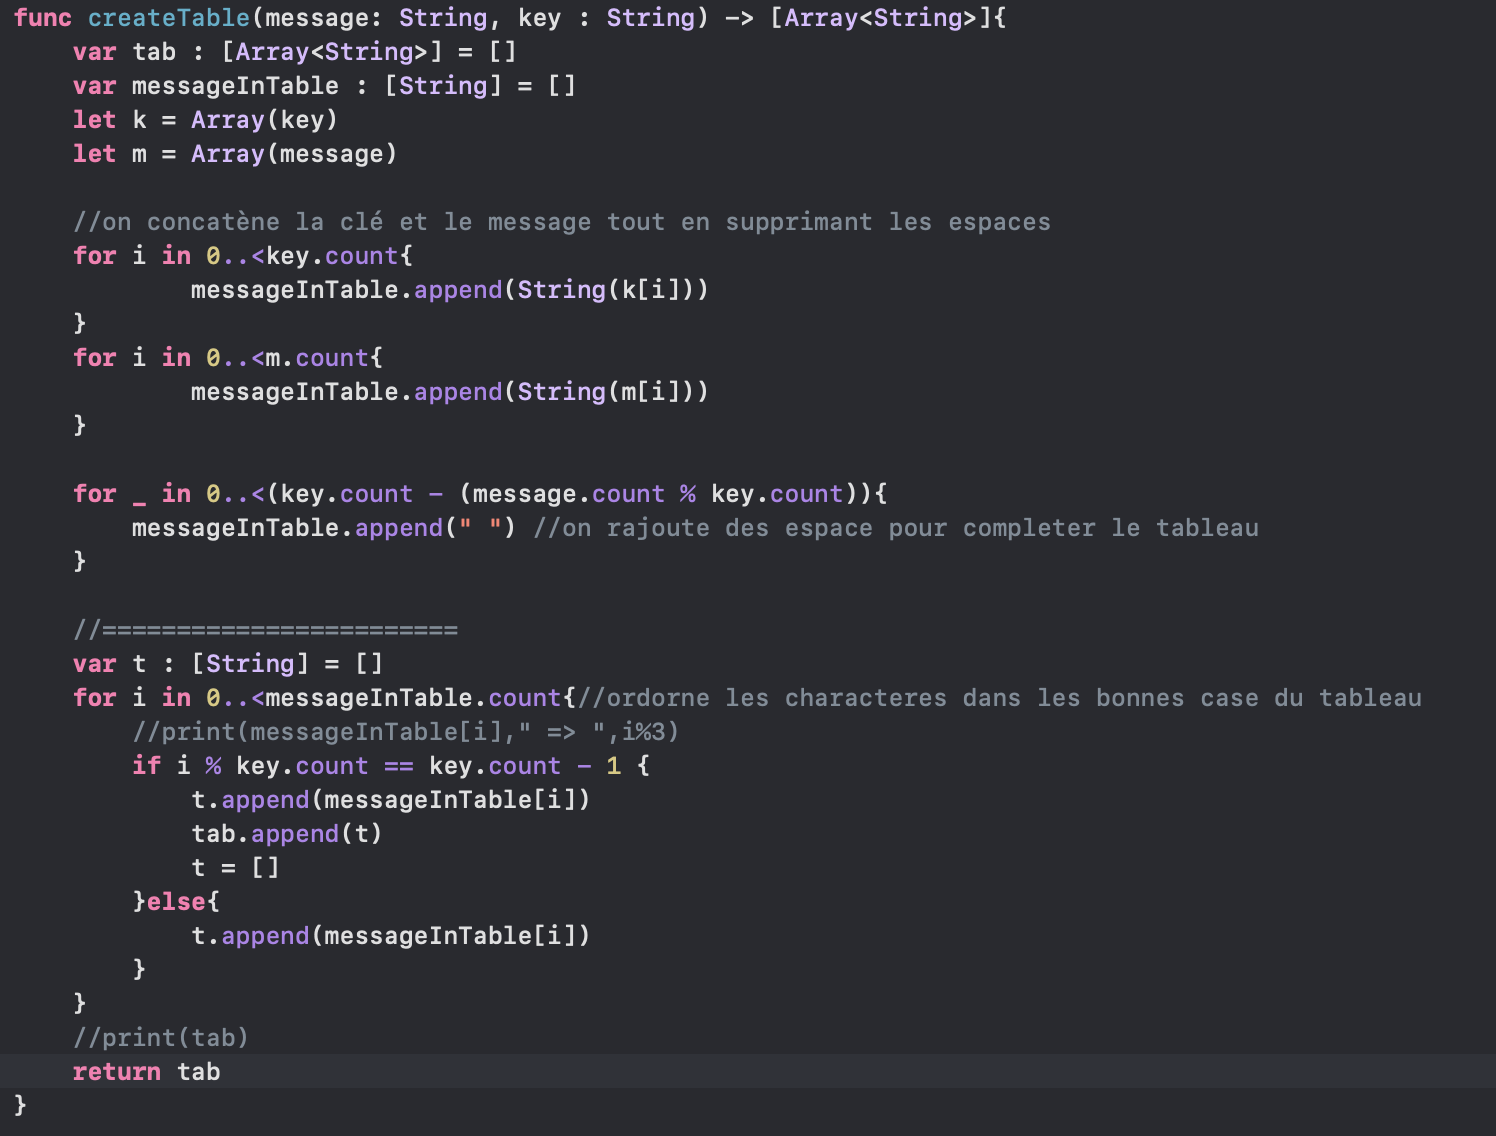
\includegraphics[scale=0.5]{Transp.png}
\end{center}
Dans ce code, nous voyons qu'on créer un tableau de tableau de type String, dont la taille est égale à la taille de la clé. On peut remarquer dans le code, que si le message ne remplit pas toutes les cases du tableau, alors on le remplissait avec un espace.
\subsection{Difficultés :}
Lors de la mise en place de cet algorithme, j'ai rencontré quelque difficulté comme par exemple :
\begin{itemize}
\item La gestion des cases vides dans le tableau
\item Gérer les occurrence afin que n'apparaissent pas les mêmes colonnes pour deux colonnes différentes.
\item La retranscription du tableau, précisément gérer les lignes avec des cases vides
\end{itemize}


\newpage
\section{DES}
\subsection{Principe :}
Le Data Encryption Standard est un algorithme de chiffrement symétrique (chiffrement par bloc) utilisant des clés de 56 bits.L'algorithme DES transforme un bloc de 64 bits en un autre bloc de 64 bits. Il manipule des clés individuelles de 56 bits, représentées par 64 bits (avec un bit de chaque octet servant pour le contrôle de parité). Ce système de chiffrement symétrique fait partie de la famille des chiffrements itératifs par blocs, plus particulièrement il s'agit d'un schéma de Feistel (du nom de Horst Feistel à l'origine du chiffrement Lucifer)... 
\url{https://fr.wikipedia.org/wiki/Data_Encryption_Standard}
\subsection{Dans le code:}
Dans cette partie, nous allons résumer l'action de chaque fonction utilisée dans l'algorithme.
La fonction prepareBloc permet de créer un ensemble de 64 bit chiffrer à partir du message.
Pour réaliser cela, elle s'appuie sur plusieurs petites fonctions permettant de transformer le message en binaire sur 64bits.\newline 
Les fonctions qui permettent de faire cela sont :
\begin{itemize}
    \item getAsciiInt (Retourne un tableau d'entier, dont chaque valeur correspond à une lettre.
\item getBinary Retourne la conversion du tableau d'entier en tableau binaire.
\item ajustOctet ajuste le nombre binaire pour être dans le format d'un octet.
\item ajustXblock ajuste l'ensemble des octets afin qu'il soit composé de 64 bits.
\item concatOctetToBloc concatène le tableau afin de retourner une chaîne de caractère.
\end{itemize}
Ensuite nous allons voir les fonctions qui gèrent la clé :
\begin{itemize}
    \item DiverseKey (retourne les 16 sous clé de K selons les sous fonctions)
\end{itemize}
\begin{center}
    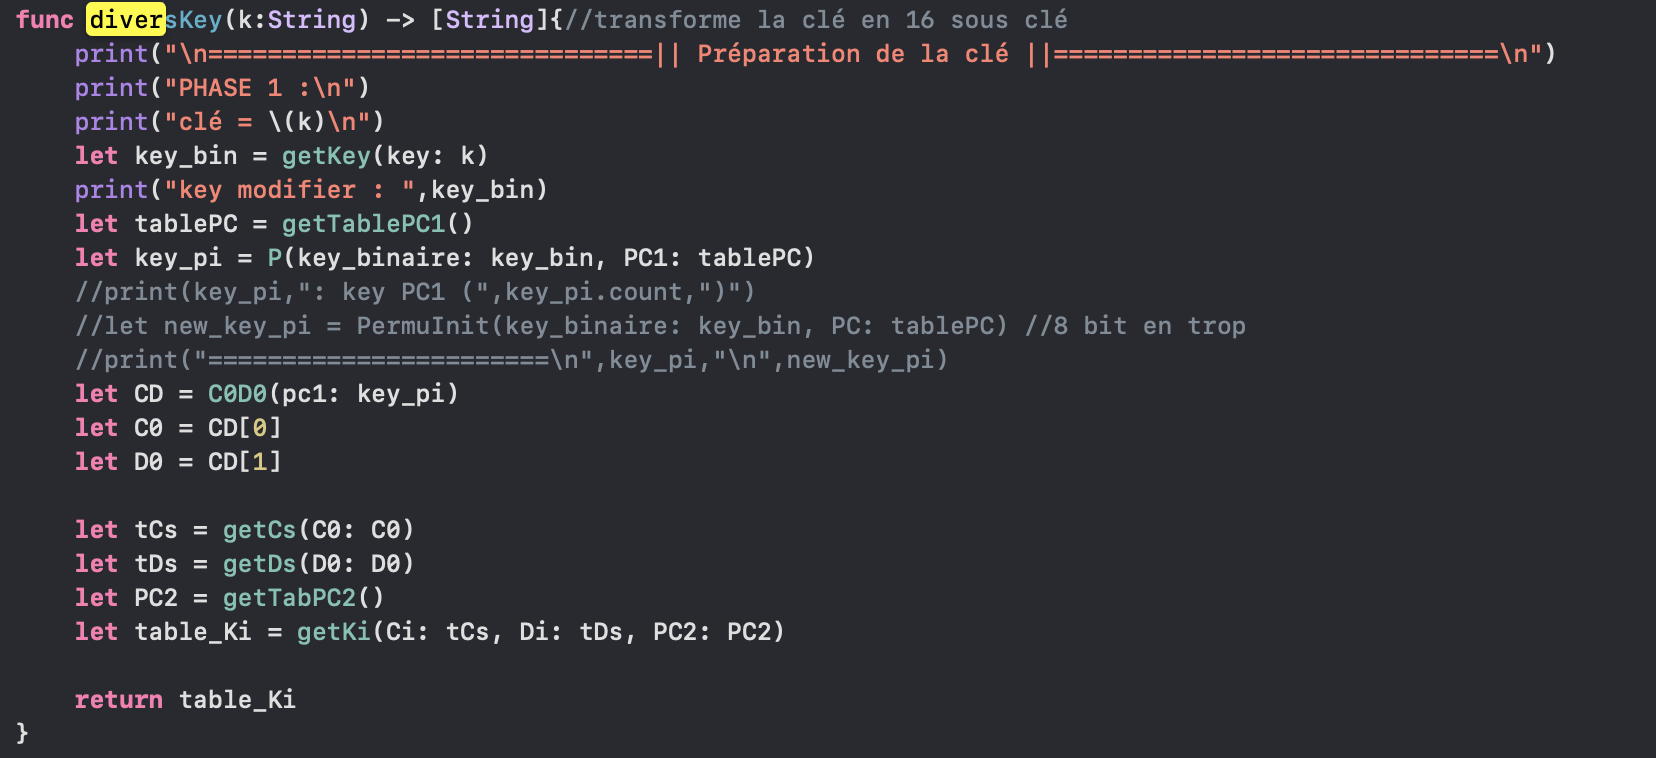
\includegraphics[scale=0.25]{DESKEY.png}
    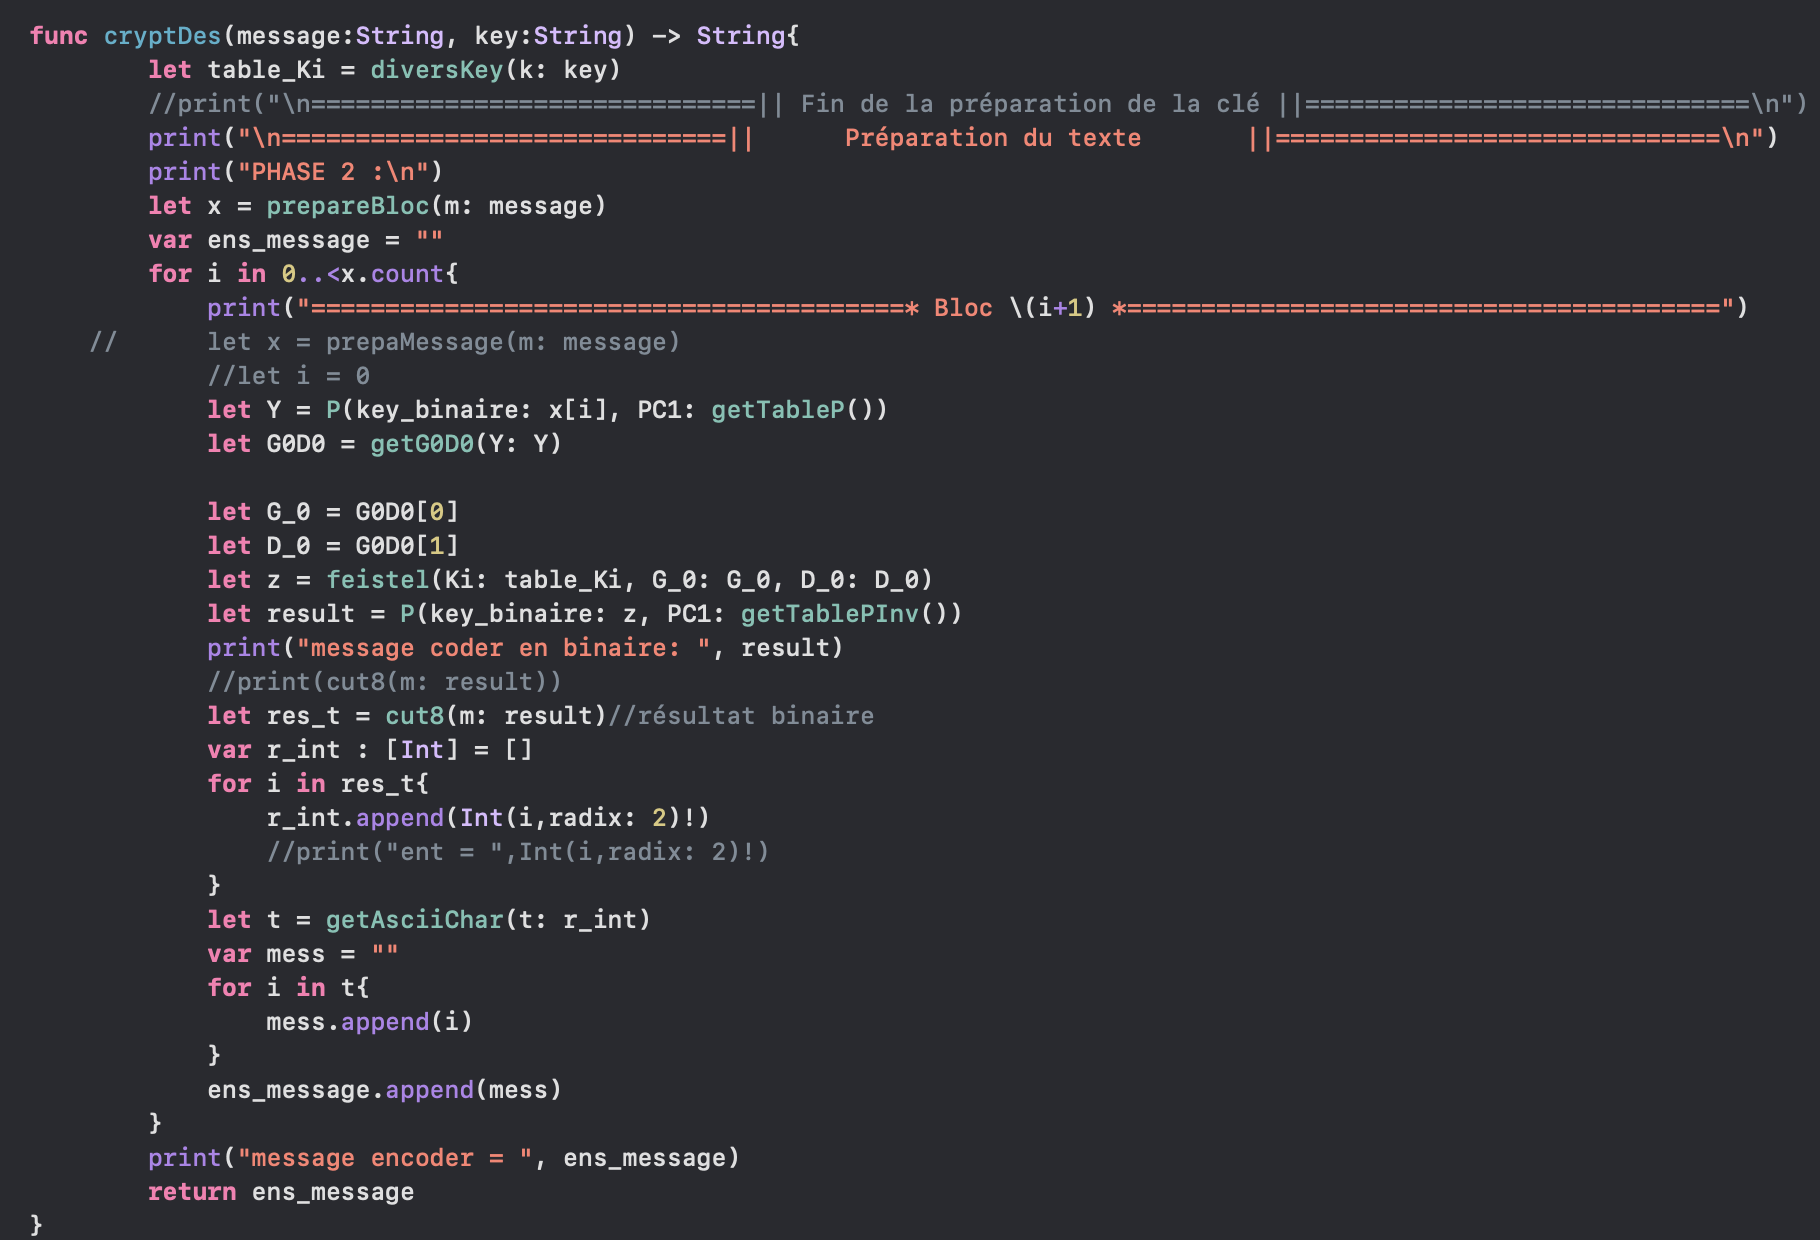
\includegraphics[scale=0.25]{DESCRYPT.png}
\end{center}
\newpage
\subsection{Difficultés :}
J'ai eu beaucoup de mal à comprendre l'algorithme du DES.
J'ai passé la plupart de mon temps dans la phase de débug afin de trouver les potentielles erreurs de mon code. Il s'avérer aussi que certains tableaux donné par le site Bibmath comportais plusieurs erreurs. 
Pour terminer, je n'ai pas réussi à debuger et à corriger la partie pour déchiffrer.
\newpage
\section{RSA}
\subsection{Principe :}
Le chiffrement RSA est un algorithme de cryptographie asymétrique, très utilisé dans le commerce électronique, et plus généralement pour échanger des données confidentielles sur Internet. Tous les calculs se font modulo un nombre entier n qui est le produit de deux nombres premiers. Le petit théorème de Fermat joue un rôle important dans la conception du chiffrement.

Les messages clairs et chiffrés sont des entiers inférieurs à l'entier n2. Les opérations de chiffrement et de déchiffrement consistent à élever le message à une certaine puissance modulo n (c'est l'opération d'exponentiation modulaire).
\subsection{Dans le code:}
\begin{center}
    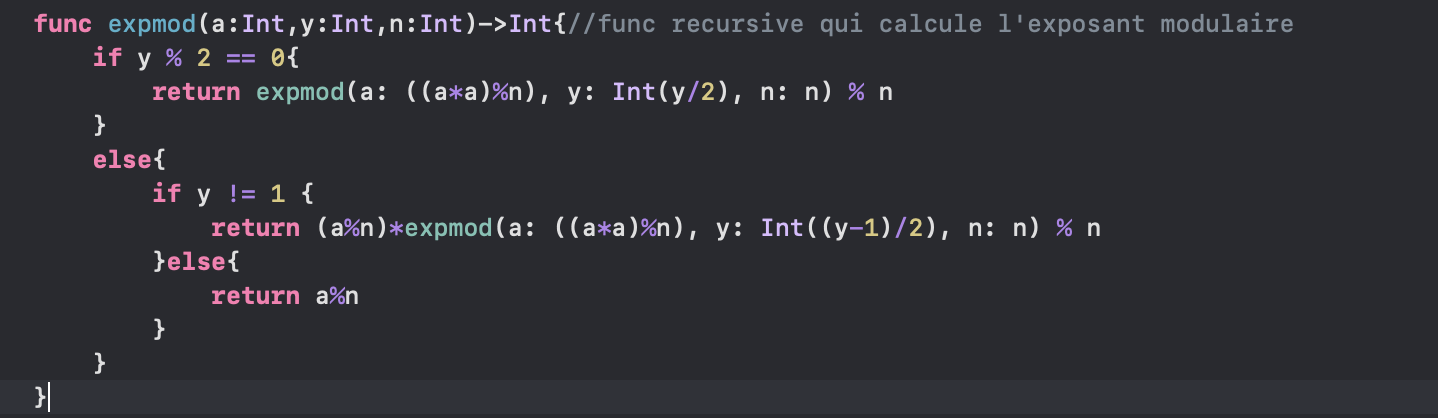
\includegraphics[scale=0.5]{EpxModRSA.png}
\end{center}
Cette fonction va nous servir à calculer la puissance modulaire, en effet, nous verrons dans le code qu'elle va servir pour coder et décoder.
\begin{center}
    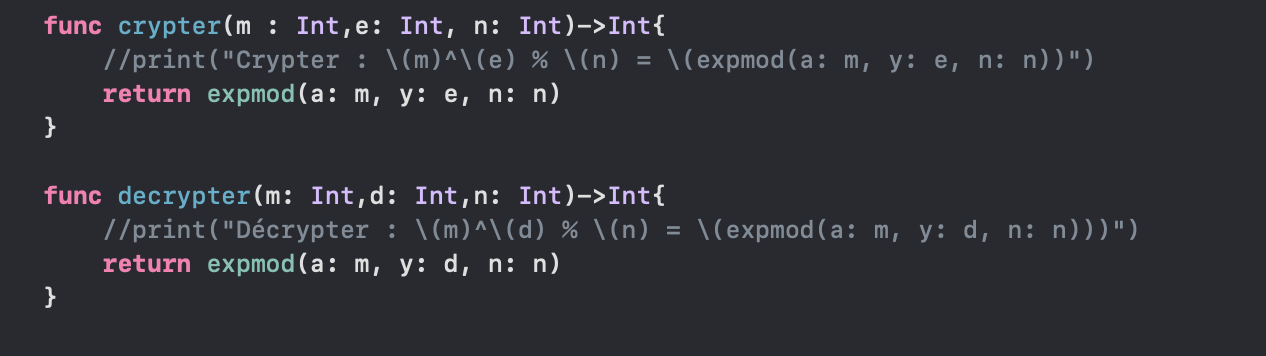
\includegraphics[scale=0.5]{CryptDecrpytRSA.png}
\end{center}
Nous allons voir ensuite comment la fonction qui permet le découpage du nombre en question.
\begin{center}
    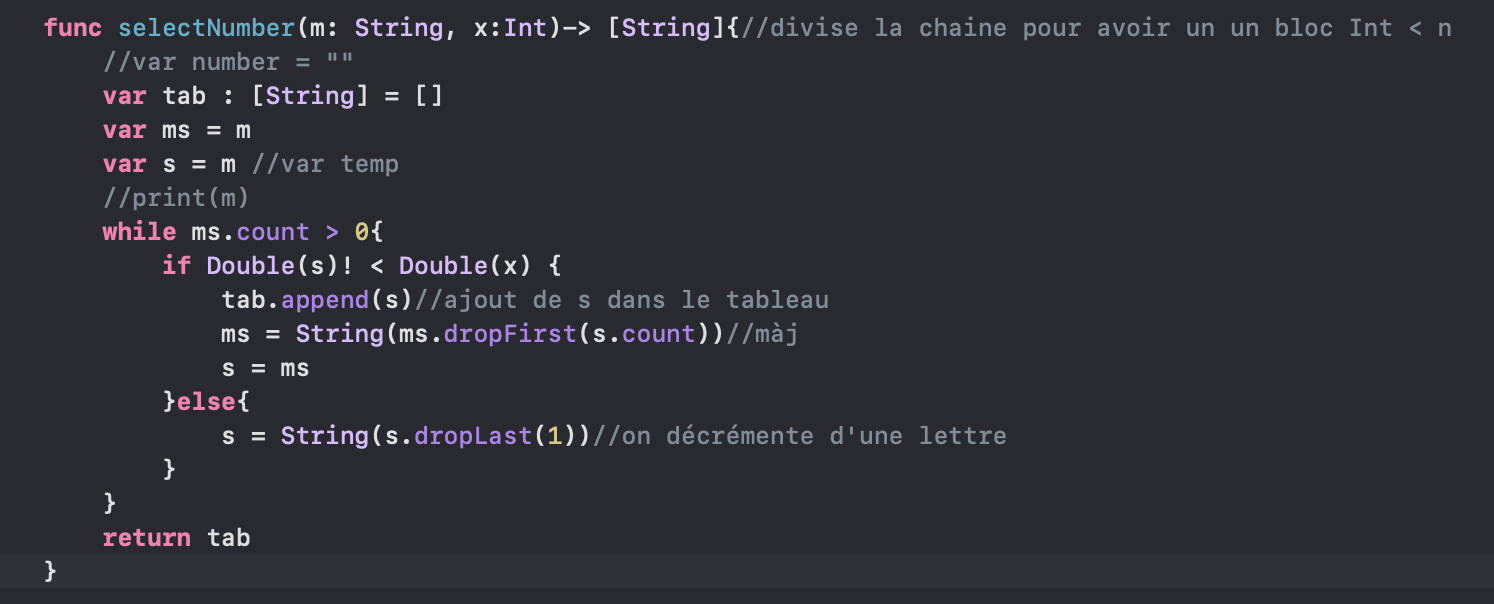
\includegraphics[scale=0.5]{SelectNRSA.png}
\end{center}
Cette fonction ci-dessus permet de voir comment le nombre est découpé pour qu'il soit inférieur à n.
\begin{center}
    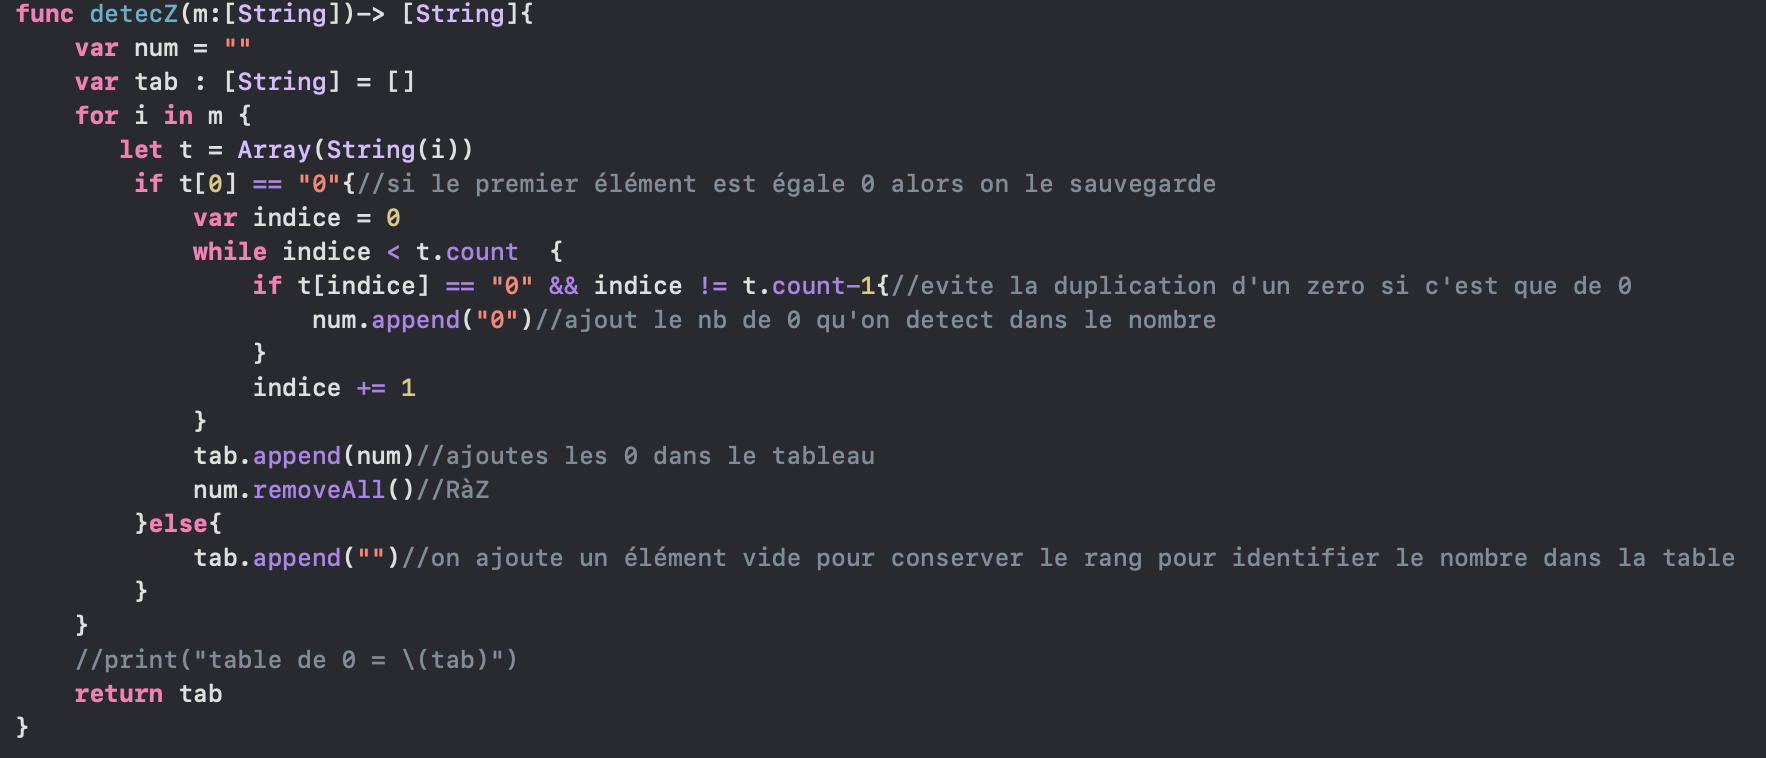
\includegraphics[scale=0.5]{DetectZRSA.png}
\end{center}
Cette fonction nous servira à détecter les zéros inutiles afin qu'ils soient sauvegardés avant d'être perdus lorsque la chaîne de caractère sera transformée en Entier.
\begin{center}
    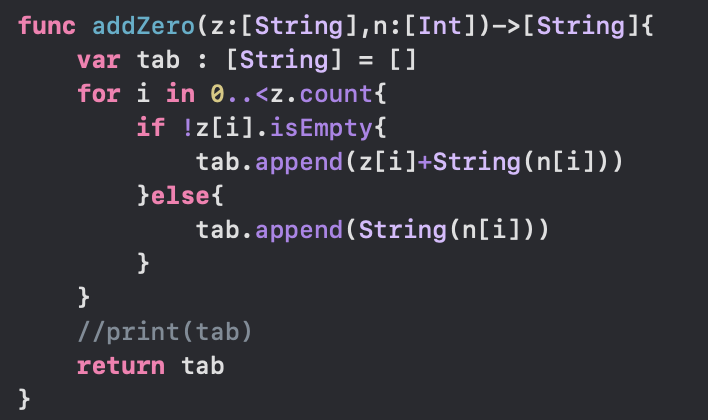
\includegraphics[scale=0.5]{addZeroRSA.png}
\end{center}
Cette fonction permet prendre les 0 stockés dans la fonction detectZero afin de bien les placée à la sortie du calcul.
Cela permet de conserver le nombre de chiffres et ensuite d'avoir une bonne restitution du message lors de la phase de décryptage.
\subsection{Difficultés :}
J'ai rencontré le plus les difficultés dans le langage Swift que pour comprendre l'algorithme.
En effet, lorsque j'utilisais la puissance avec un exposant trop grand (> 60), les valeurs retournées était arrondie.
De plus, il avait un problème lors de la conversion chaîne de caractère vers un Entier.
Précisément, lorsque nous avons "00" en chaîne de caractère, il sera traduit en 0 en Entier.
\newpage
\section{Conclusion}
Pour conclusion, je dirais que la plupart des algorithmes ont été simples pour programmer.
En effet, j'avais déjà fait la plupart des exercices en python.
De plus, il faut noter que je n'ai pas la même table ASCII que celle de l'énoncé.
\section{Bibliographie}
\begin{itemize}
    \item \url{https://www.ascii-code.com/?fbclid=IwAR0jwjK80nSHUvUrkpcmGVm0dMY4Tv2MQCRuesuB2FbhOqtLZnZSsFBZCqU}
    \item \url{http://www.bibmath.net/crypto/index.php?action=affiche&quoi=moderne/des}
    \item \url{https://fr.wikipedia.org/wiki/Constantes_du_DES}
    \item \url{https://www.univers-ti-nspire.fr/files/pdf/05-exponentiation_modulaire-TNS21.pdf}
    \item \url{https://www.youtube.com/watch?v=aYI9B9ra_P4}
    \item \url{https://fr.wikipedia.org/wiki/Chiffrement_RSA#Fonctionnement_détaillé}
    \item \url{https://fr.wikipedia.org/wiki/Algorithme_d%27Euclide}
\end{itemize}








\end{document}
